% Results fragment. Requires graphicx, float and booktabs.
% The supplied Summary is preserved separately in Summary-unchanged.tex.
\section{Results}\label{Results}

This section compares the userspace and in-kernel implementations on the supplied FABRIC recordings. It covers memory, CPU utilization, observed throughput, local decision timing and detection quality. Resource measurements describe one recording per implementation and blocking setting, with separate accuracy runs. Replay timing and build differences limit causal or statistical claims. These recordings do not establish results for the other proposed testbed or all six planned datasets.

\subsection{Attack visualization}

Figure~\ref{fig:traffic} shows an example with kernel detection and blocking enabled. The observed workload has an initial low-rate period of approximately 14 minutes, a high-rate flood lasting approximately 12 minutes, and a lower-rate tail for the remainder of the roughly 44-minute recording. These phases describe the measured traffic rate. In particular, a low packet rate does not establish that the traffic is benign according to the dataset labels.

\begin{figure}[H]
    \centering
    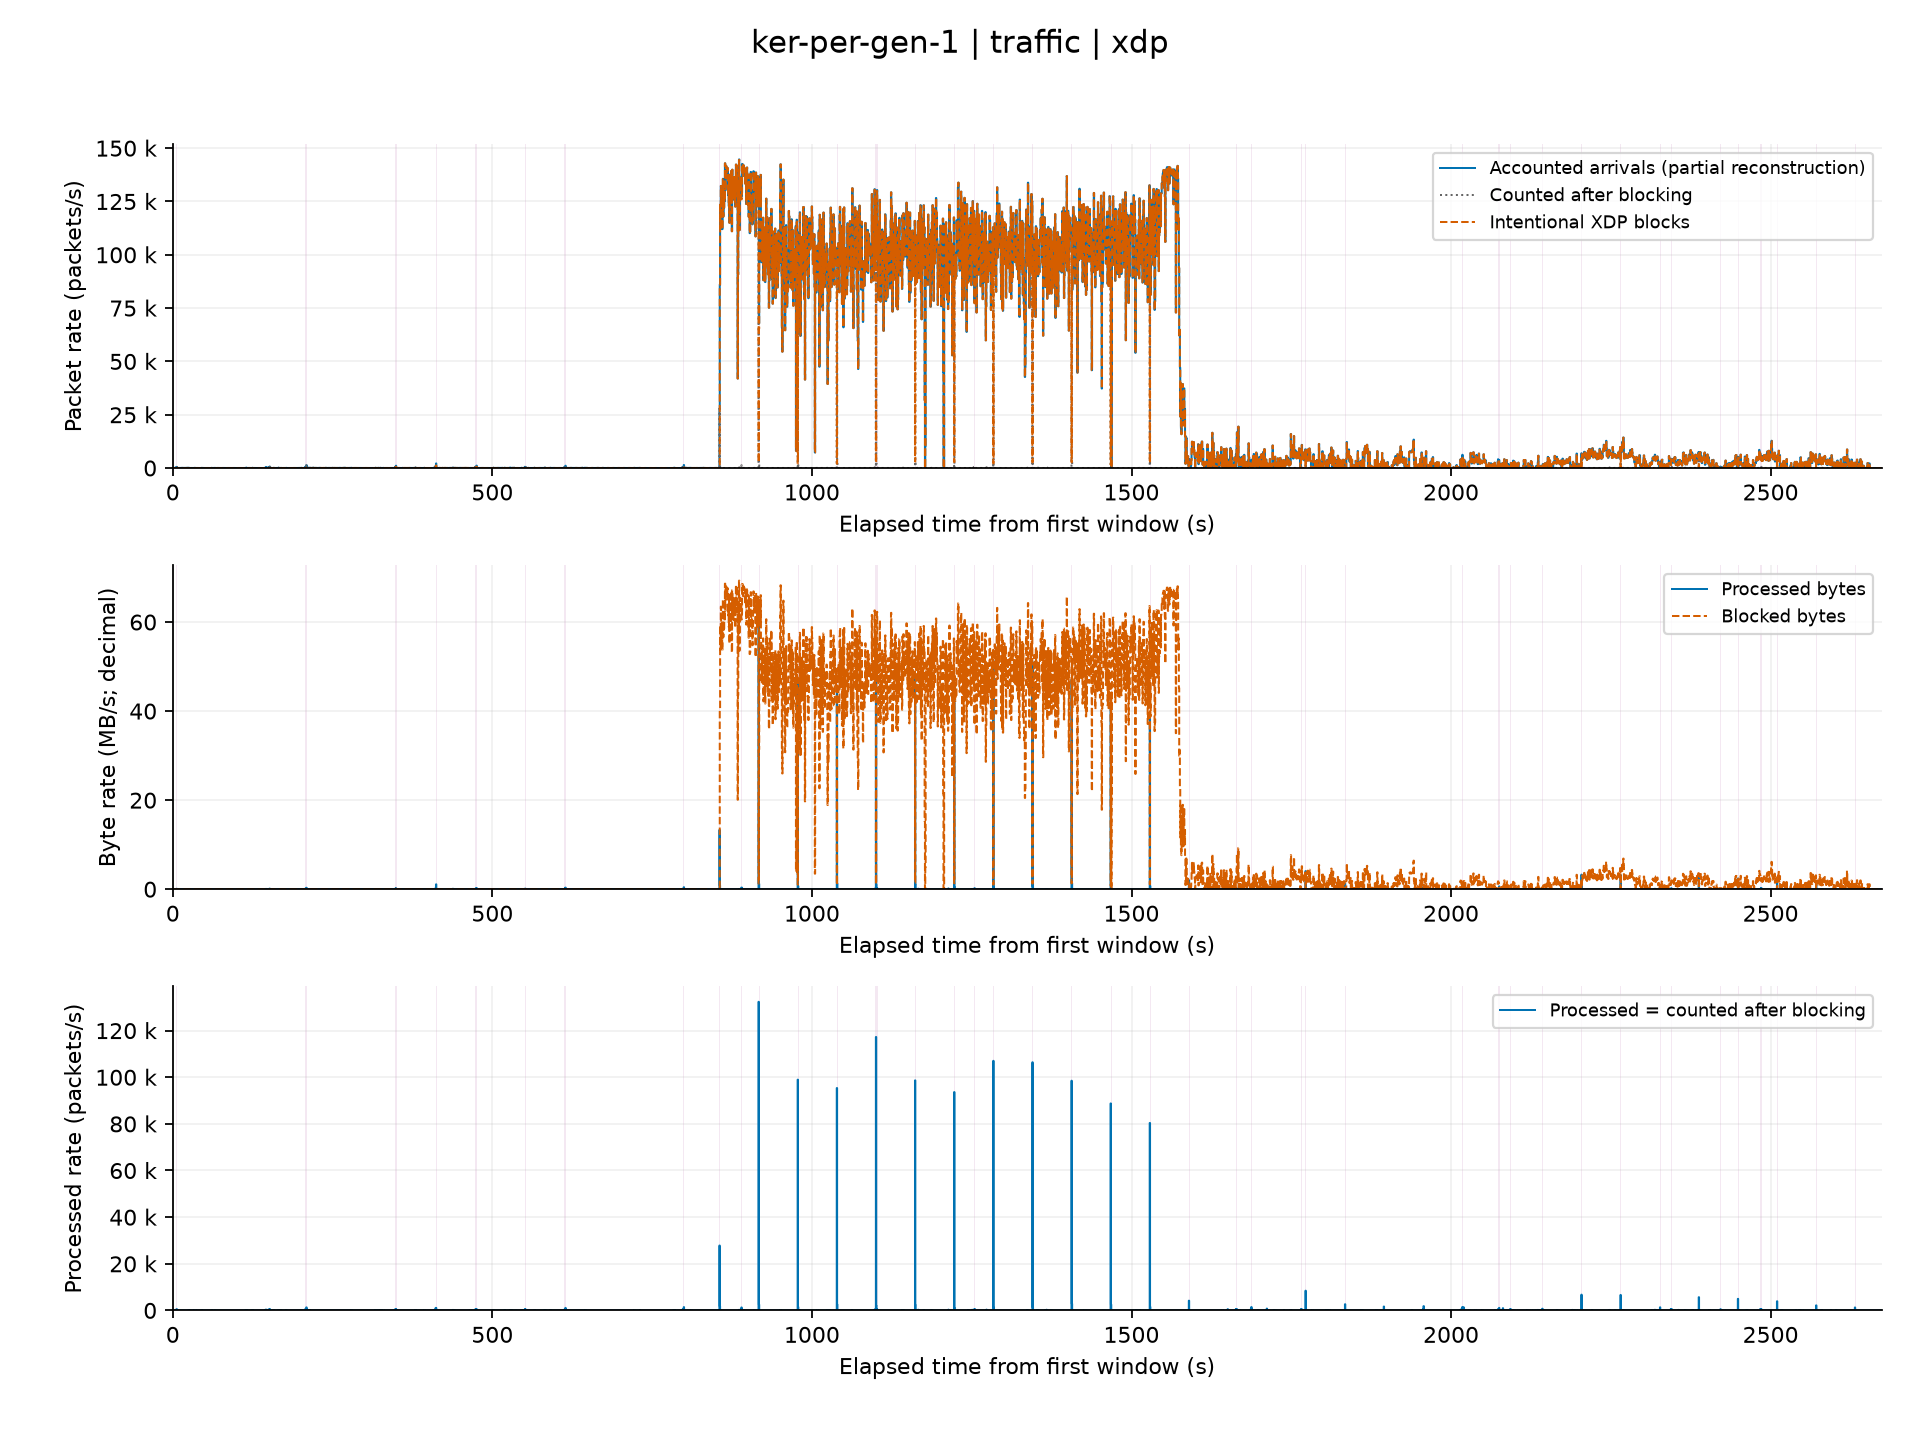
\includegraphics[width=.88\textwidth]{resources/testing-figures/traffic-ker-blk.png}
    \caption{Traffic during kernel detection with blocking enabled. The panels show packet accounting, processed and blocked byte rates, and the residual packet rate after blocking. Byte rates are decimal MB/s.}
    \label{fig:traffic}
\end{figure}

During the high-rate phase, arrivals commonly reach approximately 100,000--140,000 packets/s and 40--70~MB/s. Most accounted packets are intentionally blocked. The lower panel reveals brief bursts that still reach the counting stage, consistent with traffic being admitted when blocklist entries expire before being renewed. Purple shading marks the detector's malicious-window verdicts; it is not an independent ground-truth annotation.

The arrival series reconstructs local counted and blocked traffic and excludes upstream losses. Processed packets already exclude blocks; subtracting blocked packets again would be incorrect. Residual traffic does not establish legitimate-service availability.

\clearpage
\subsection{Memory utilization}

Memory measurements were collected to assess whether moving packet counting into the kernel reduced the detector's memory footprint. The blue line is the cgroup's \texttt{anon + kernel + sock} memory, in binary MiB. The grey line is \texttt{memory.current}, which also includes file cache. Where available, the orange line adds separately charged BPF map memory to the blue line; program and JIT memory are outside that addition. These quantities describe the detector's recorded footprint, rather than total host RAM utilization.

\begin{figure}[H]
    \centering
    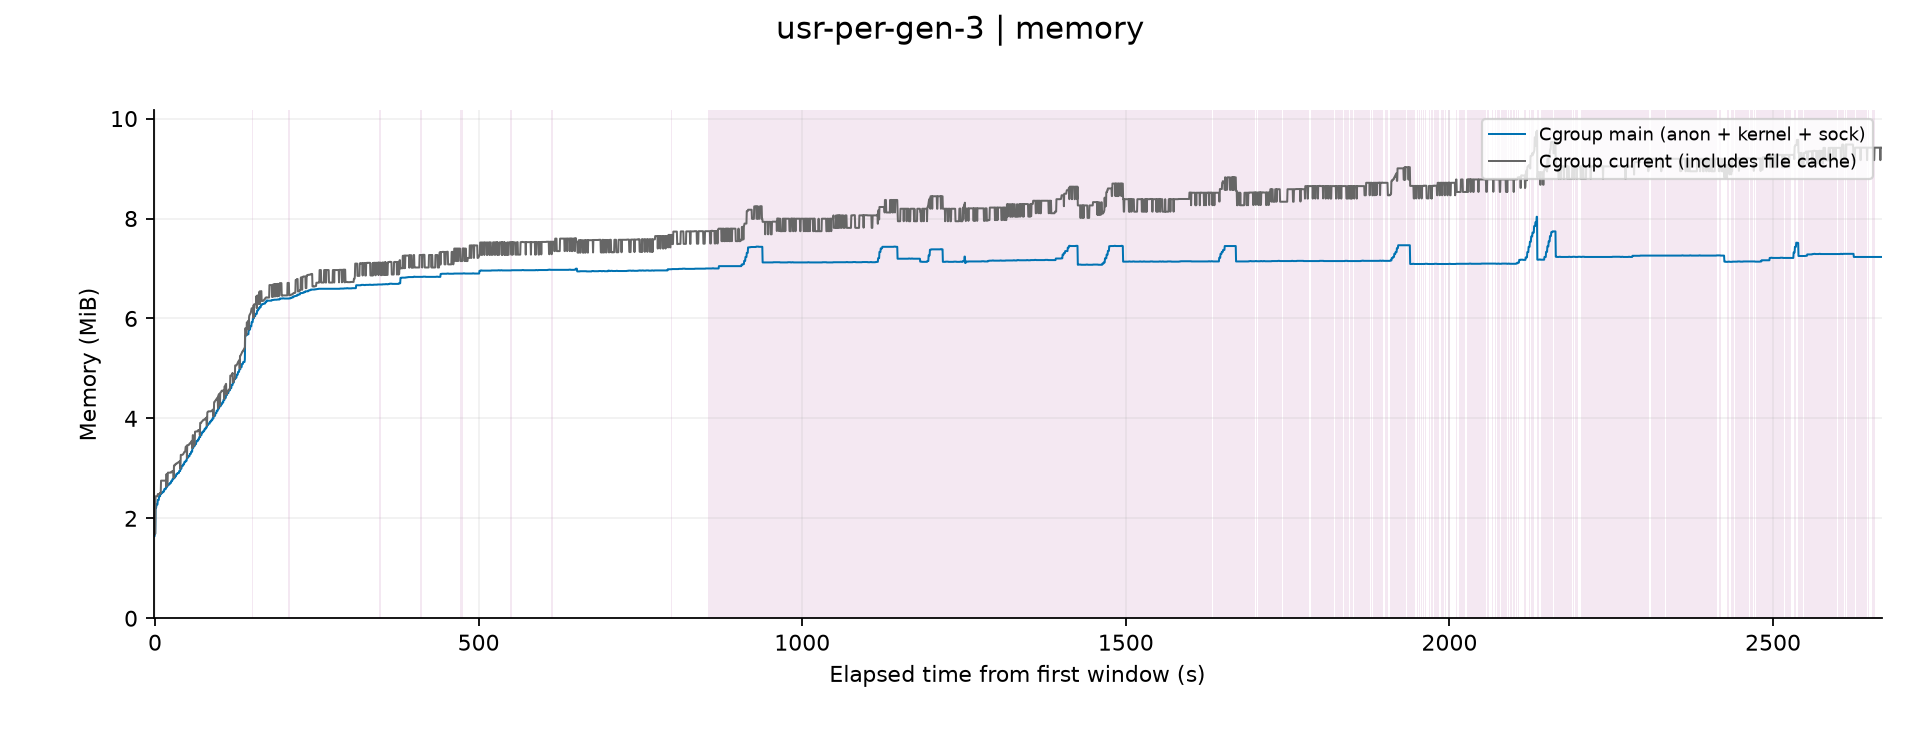
\includegraphics[width=\textwidth]{resources/testing-figures/memory-usr-unblk.png}
    \par\smallskip
    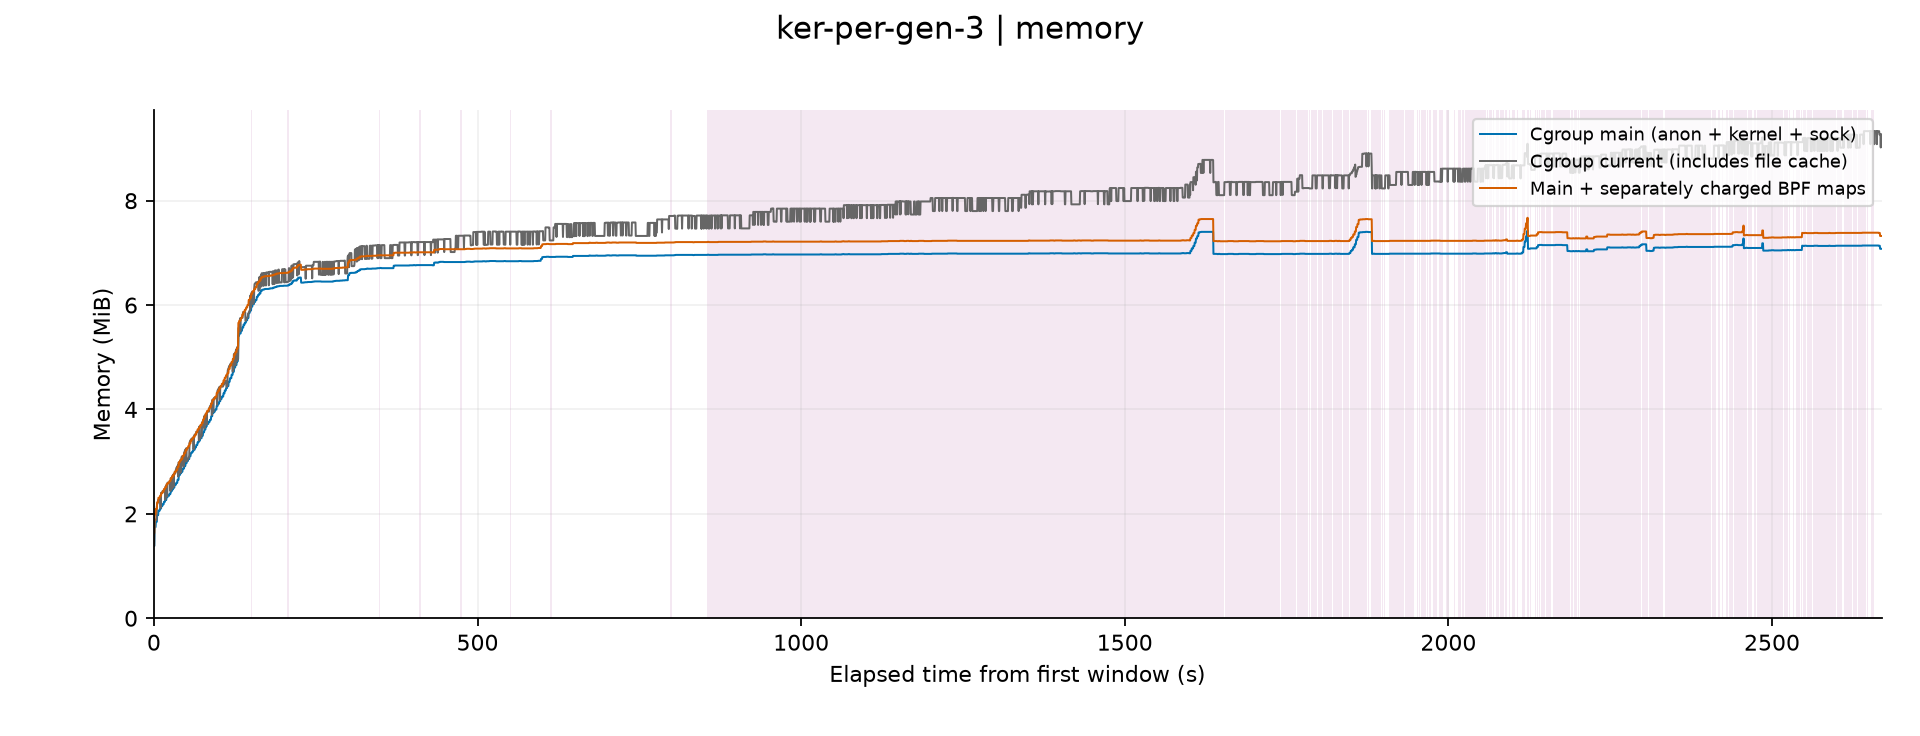
\includegraphics[width=\textwidth]{resources/testing-figures/memory-ker-unblk.png}
    \caption{Memory with blocking disabled: userspace above and kernel below. The panels use independent vertical scales.}
    \label{fig:memory-unblk}
\end{figure}

Both implementations show an initial rise from approximately 2~MiB, followed by a much flatter main-memory footprint near 7~MiB. The whole-recording median main memory is 7.13~MiB for userspace and 6.98~MiB for the kernel implementation. The kernel maps add approximately 0.246~MiB, giving a median of 7.23~MiB for main memory plus recorded maps. An equivalent combined total is unavailable for the unblocked userspace recording because its separately charged map footprint was not confirmed.

The steadily increasing grey curves should not be interpreted as equivalent growth in the detector's active data structures. Main memory remains comparatively stable while the difference between \texttt{current} and main memory increases; file cache is included in that difference. The high-rate flood produces no large sustained increase in main memory. These plots therefore provide no clear evidence of a substantial memory reduction from the kernel implementation.

\clearpage
\begin{figure}[H]
    \centering
    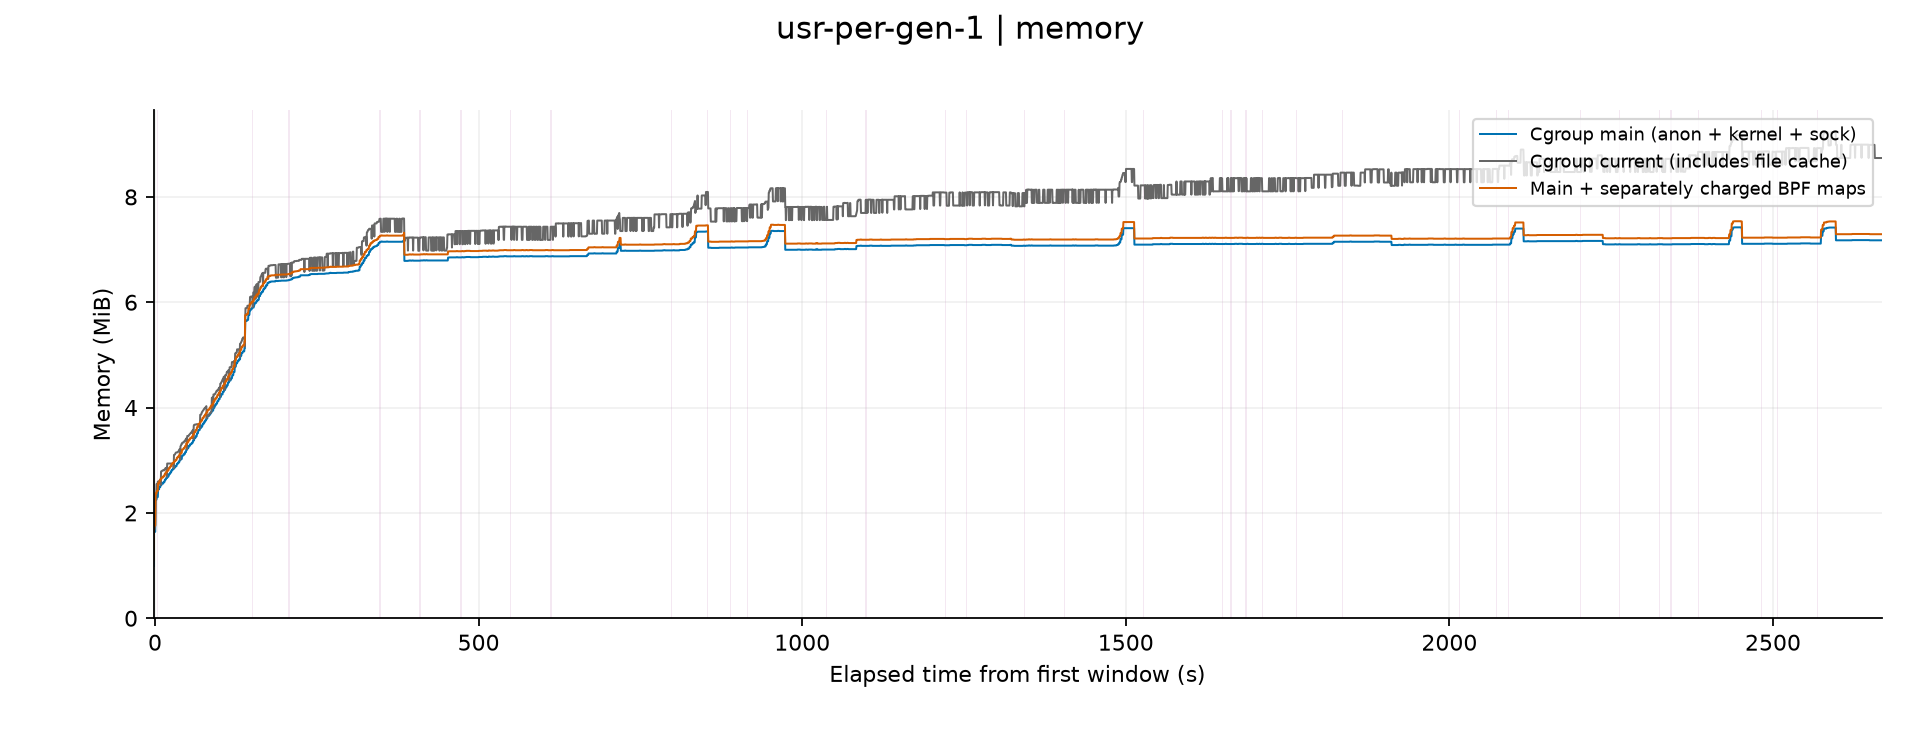
\includegraphics[width=\textwidth]{resources/testing-figures/memory-usr-blk.png}
    \par\smallskip
    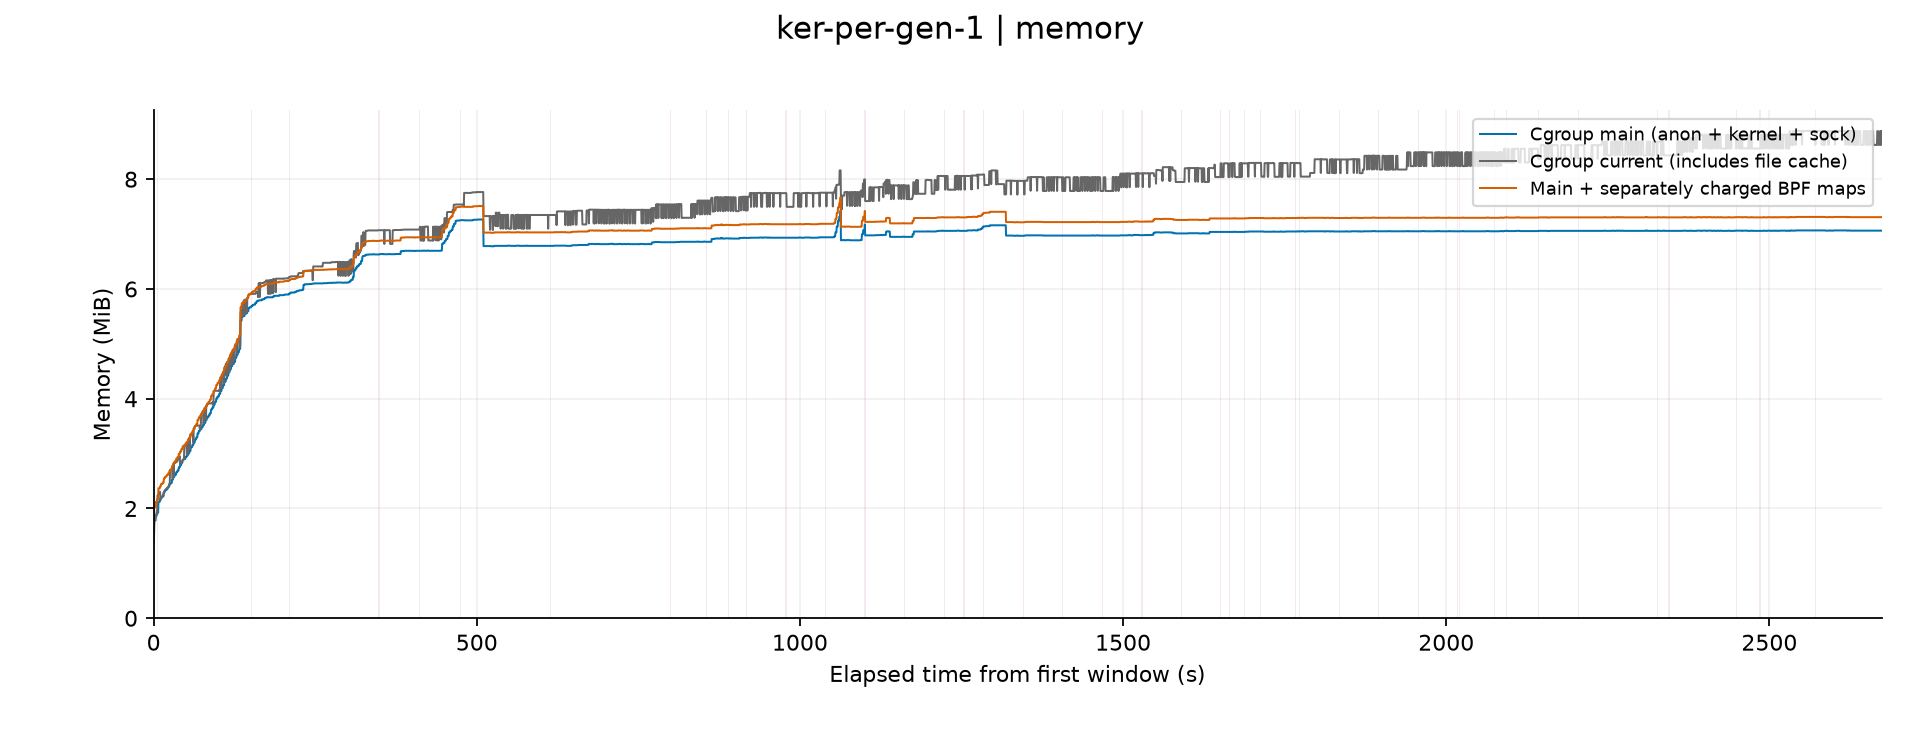
\includegraphics[width=\textwidth]{resources/testing-figures/memory-ker-blk.png}
    \caption{Memory with blocking enabled: userspace above and kernel below. Orange includes the stable, separately charged map footprint recorded for each implementation.}
    \label{fig:memory-blk}
\end{figure}

With blocking enabled, the main-memory median is again approximately 7~MiB in both implementations (Table~\ref{tab:memory}). The kernel implementation has a slightly smaller main-memory median, but its larger map footprint reverses this small difference when maps are included. The combined medians are 7.20~MiB for userspace and 7.26~MiB for the kernel implementation. This difference is small and does not support a claim of improved memory efficiency.

\begin{table}[H]
    \centering
    \small
    \begin{tabular}{llrr}
        \toprule
        Blocking & Implementation & Main median (MiB) & Main + maps median (MiB) \\
        \midrule
        Disabled & Userspace & 7.13 & Unavailable \\
        Disabled & Kernel & 6.98 & 7.23 \\
        Enabled & Userspace & 7.09 & 7.20 \\
        Enabled & Kernel & 7.01 & 7.26 \\
        \bottomrule
    \end{tabular}
    \caption{Sample-based memory medians over each complete recording, including startup. Blocking uses 121,832~bytes of separately charged maps for userspace and 257,600~bytes for the kernel implementation.}
    \label{tab:memory}
\end{table}

Early packet drops may avoid transient allocations elsewhere in the network stack, but these cgroup measurements do not isolate that host-wide effect. The absence of a clear reduction in the recorded detector footprint therefore does not establish whether total network-stack memory changed.

\clearpage
\subsection{CPU utilization}

Whole-host CPU and process CPU measure different parts of the work. Host utilization is the busy share across all CPU cores and includes XDP processing, network-stack activity and unrelated processes. Detector-process utilization uses one core as its denominator, so 100\% means one fully occupied core. It excludes per-packet XDP work. Host utilization is consequently the more useful of these two measurements for assessing the total effect of moving counting into the kernel.

\subsubsection{Whole-host CPU with blocking disabled}

\begin{figure}[H]
    \centering
    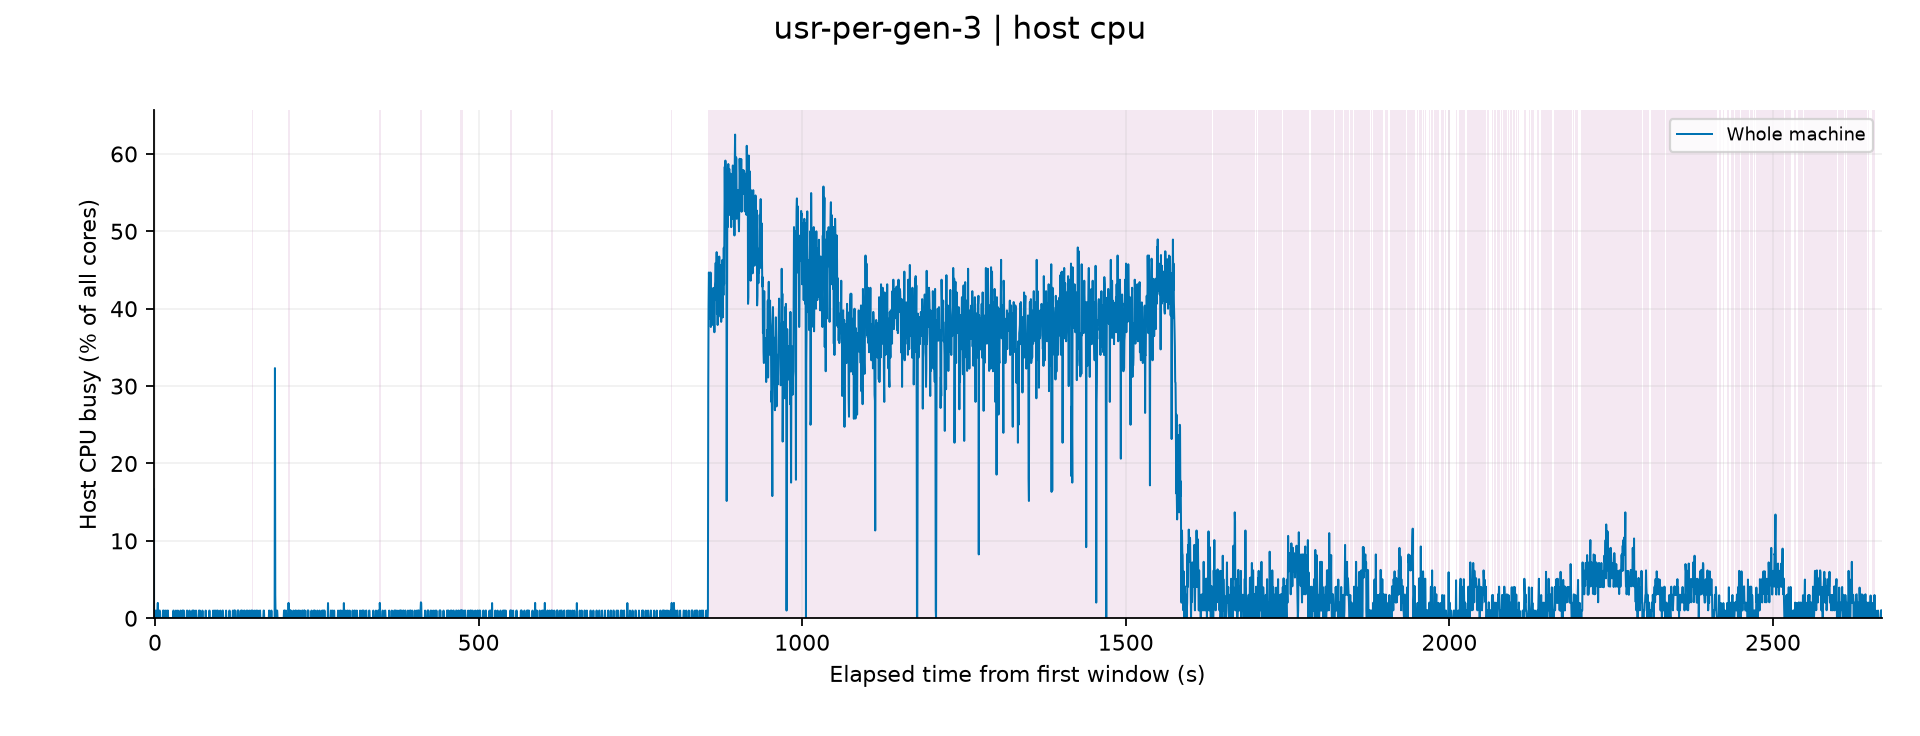
\includegraphics[width=\textwidth]{resources/testing-figures/host_cpu-usr-unblk.png}
    \par\smallskip
    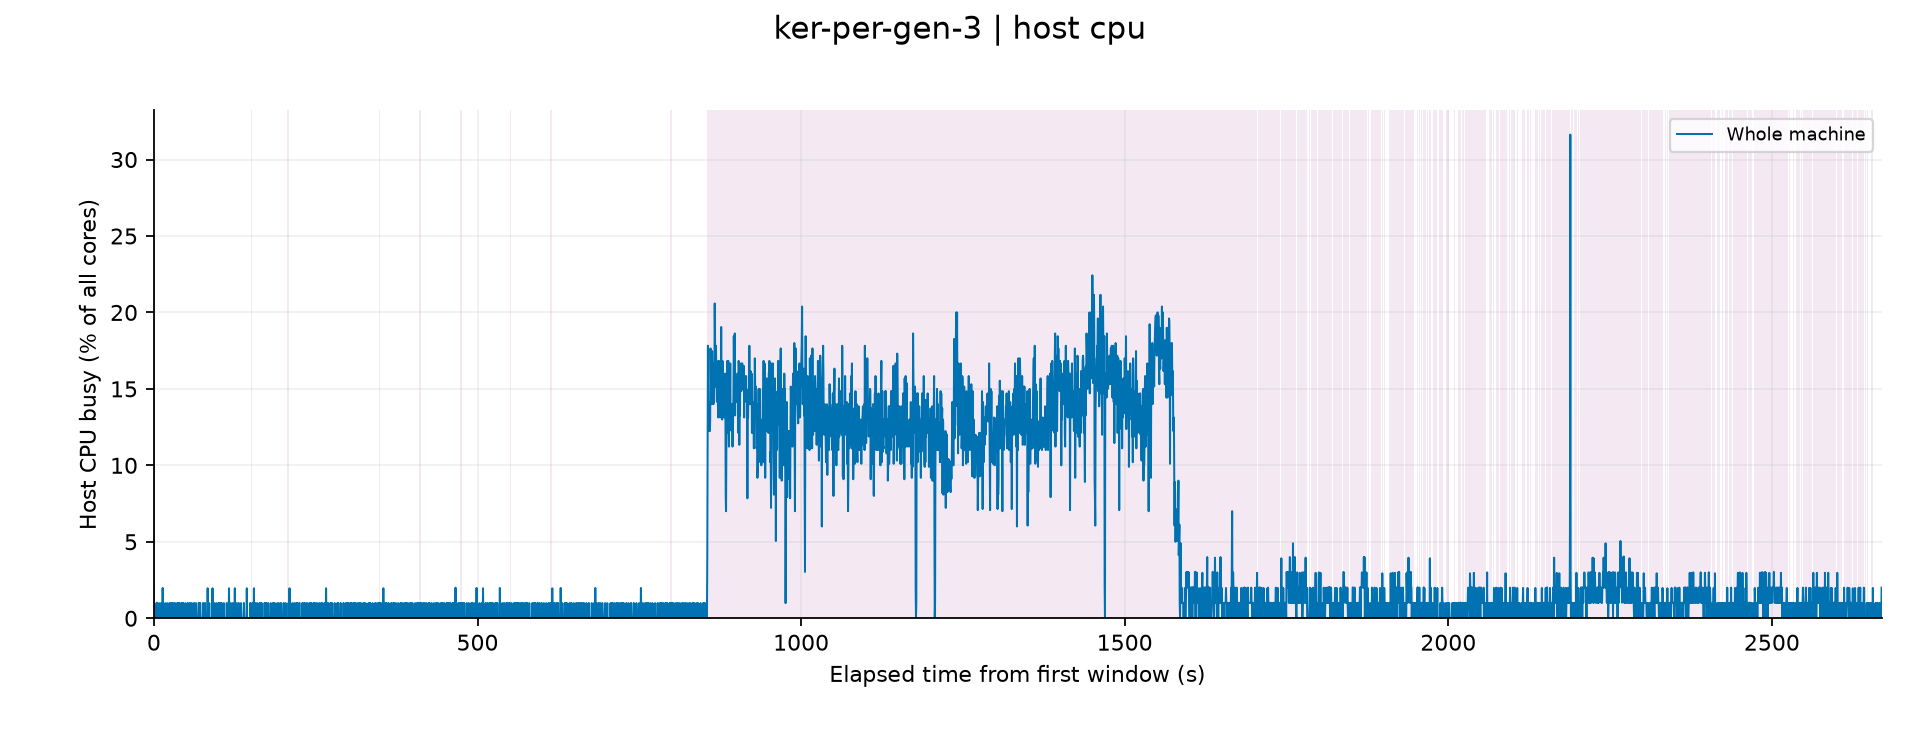
\includegraphics[width=\textwidth]{resources/testing-figures/host_cpu-ker-unblk.png}
    \caption{Whole-host CPU with blocking disabled: userspace above and kernel below. Percentages refer to all cores, and the vertical scales differ.}
    \label{fig:cpu-host-unblk}
\end{figure}

Before the flood, host utilization is generally around 1\% or lower, apart from isolated spikes. The difference becomes clear during the high-rate phase. Over the approximate elapsed interval 850--1575~s, counter-weighted host utilization is 38.95\% for userspace and 13.44\% for the kernel implementation. This is a descriptive reduction of approximately 65\% in these recordings. Both curves fall sharply when the packet rate decreases, with the kernel curve generally remaining lower during the tail.

These results are consistent with a lower host CPU cost when counting is performed at XDP. They do not isolate detector overhead, because a same-traffic run without a detector was not provided. The selected intervals follow the visible high-rate phase on each local clock and have not been validated against a common replay timeline.

\clearpage
\subsubsection{Whole-host CPU with blocking enabled}

\begin{figure}[H]
    \centering
    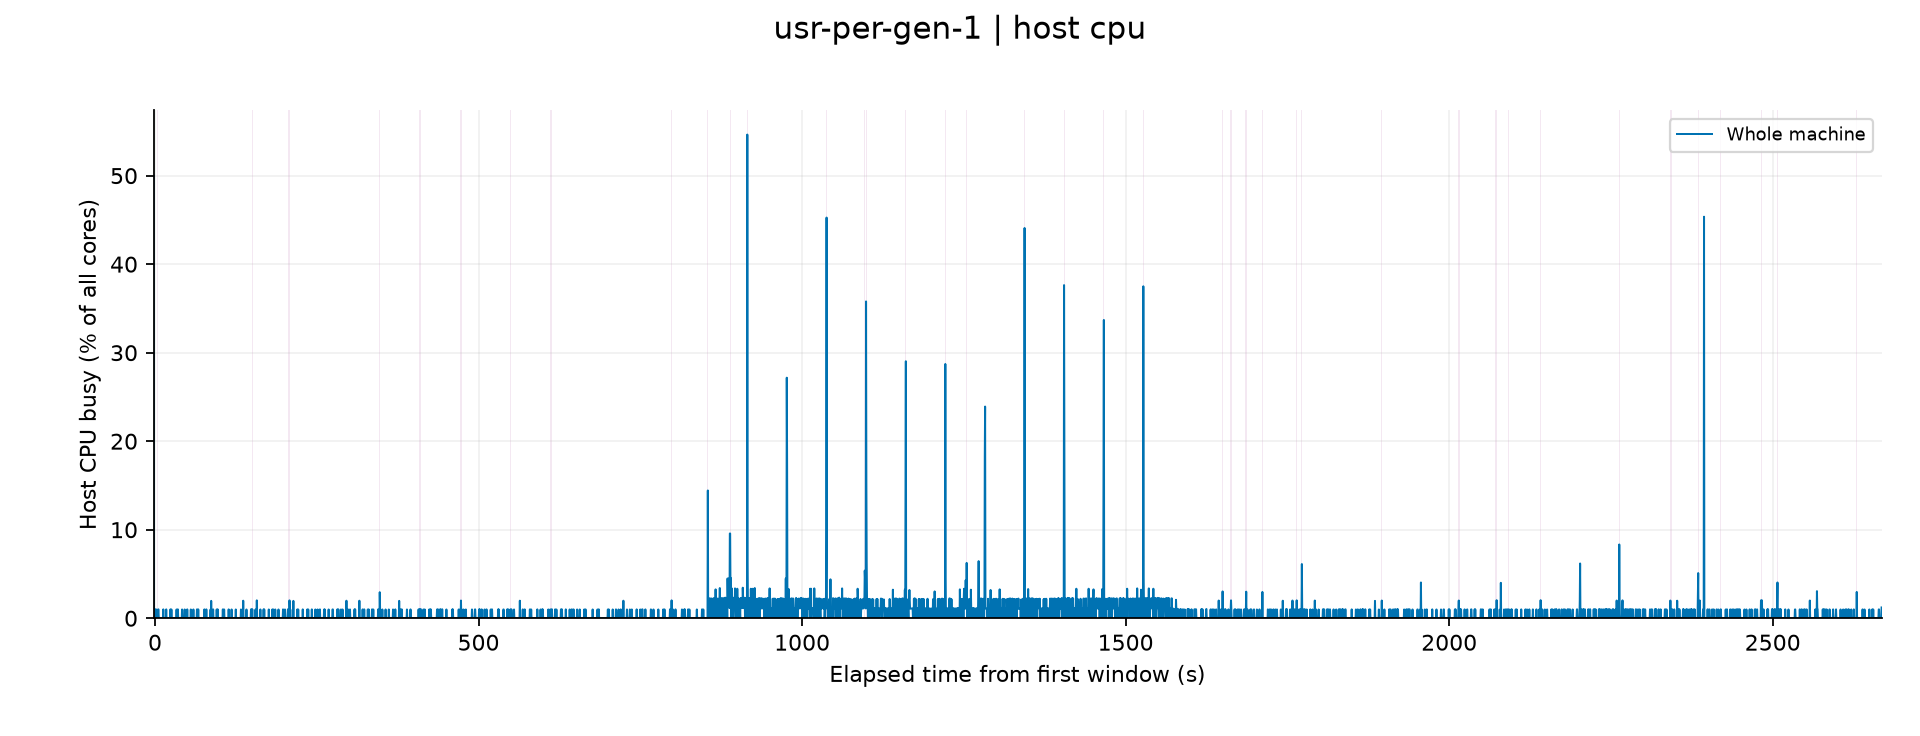
\includegraphics[width=\textwidth]{resources/testing-figures/host_cpu-usr-blk.png}
    \par\smallskip
    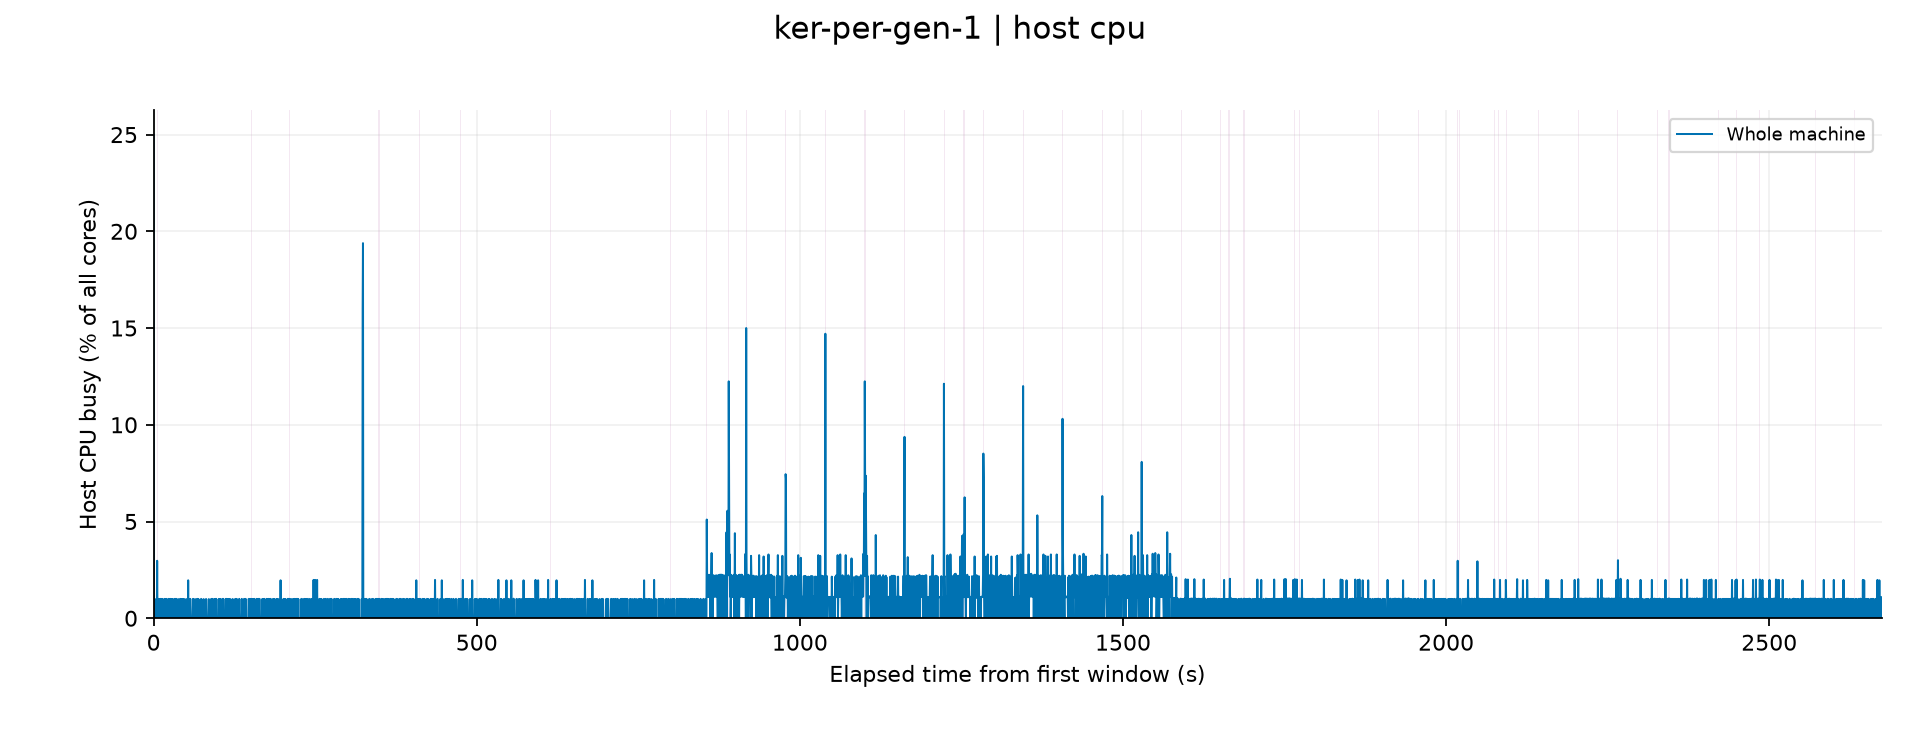
\includegraphics[width=\textwidth]{resources/testing-figures/host_cpu-ker-blk.png}
    \caption{Whole-host CPU with blocking enabled: userspace above and kernel below. Most packets are intentionally dropped, leaving low sustained CPU use with intermittent bursts.}
    \label{fig:cpu-host-blk}
\end{figure}

Enabling blocking removes most sustained counting work in both implementations. Over the approximate high-rate interval, host utilization is 1.53\% for userspace and 1.32\% for kernel detection. The userspace plot contains larger short bursts, reaching approximately 55\% over the complete recording, while the kernel recording peaks at 25\%. Their recurrence during the flood is consistent with the one-minute blocklist lifetime and the bursts of packets admitted before a renewed block.

Whole-recording averages are much smaller because they include the quiet initial period and lower-rate tail (Table~\ref{tab:cpu}). On that population the kernel average is slightly higher, so the results do not support an overall average CPU advantage with blocking enabled. Both implementations enforce their blocklists through XDP; the userspace baseline therefore also benefits from early drops.

\begin{table}[H]
    \centering
    \small
    \begin{tabular}{llrr}
        \toprule
        Blocking & Implementation & Whole recording (\%) & High-rate phase (\%) \\
        \midrule
        Disabled & Userspace & 11.46 & 38.95 \\
        Disabled & Kernel & 4.14 & 13.44 \\
        Enabled & Userspace & 0.52 & 1.53 \\
        Enabled & Kernel & 0.58 & 1.32 \\
        \bottomrule
    \end{tabular}
    \caption{Counter-weighted host CPU utilization. The approximate high-rate phase uses samples ending between 850 and 1575~s on each recording's local clock. Whole-recording values include startup and quiet traffic.}
    \label{tab:cpu}
\end{table}

\clearpage
\subsubsection{Detector-process CPU}

\begin{figure}[H]
    \centering
    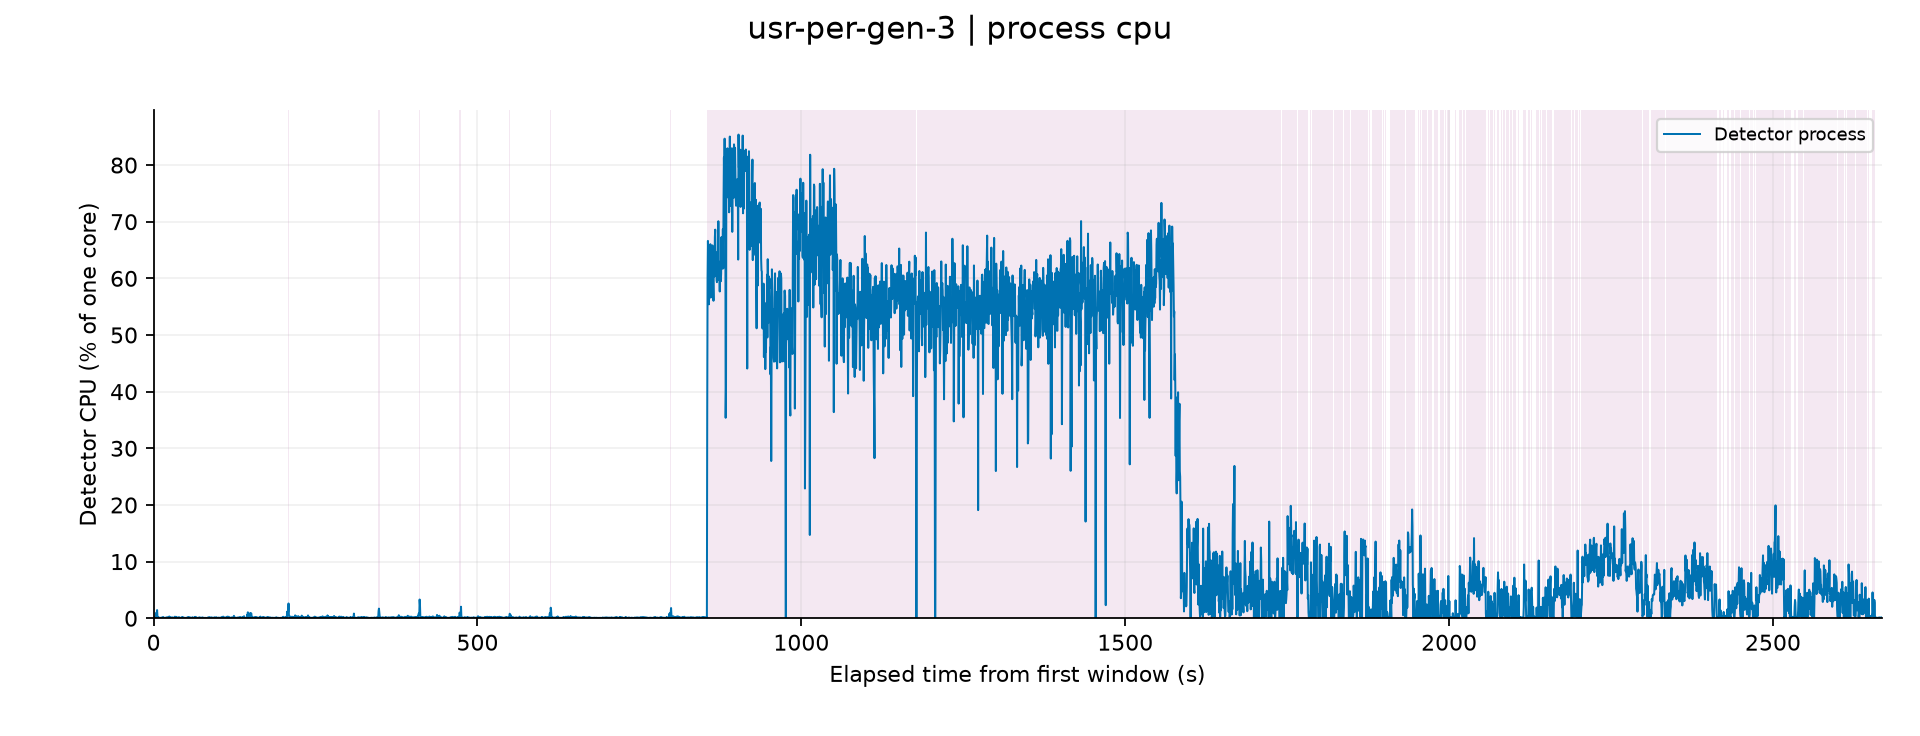
\includegraphics[width=\textwidth]{resources/testing-figures/process_cpu-usr-unblk.png}
    \par\smallskip
    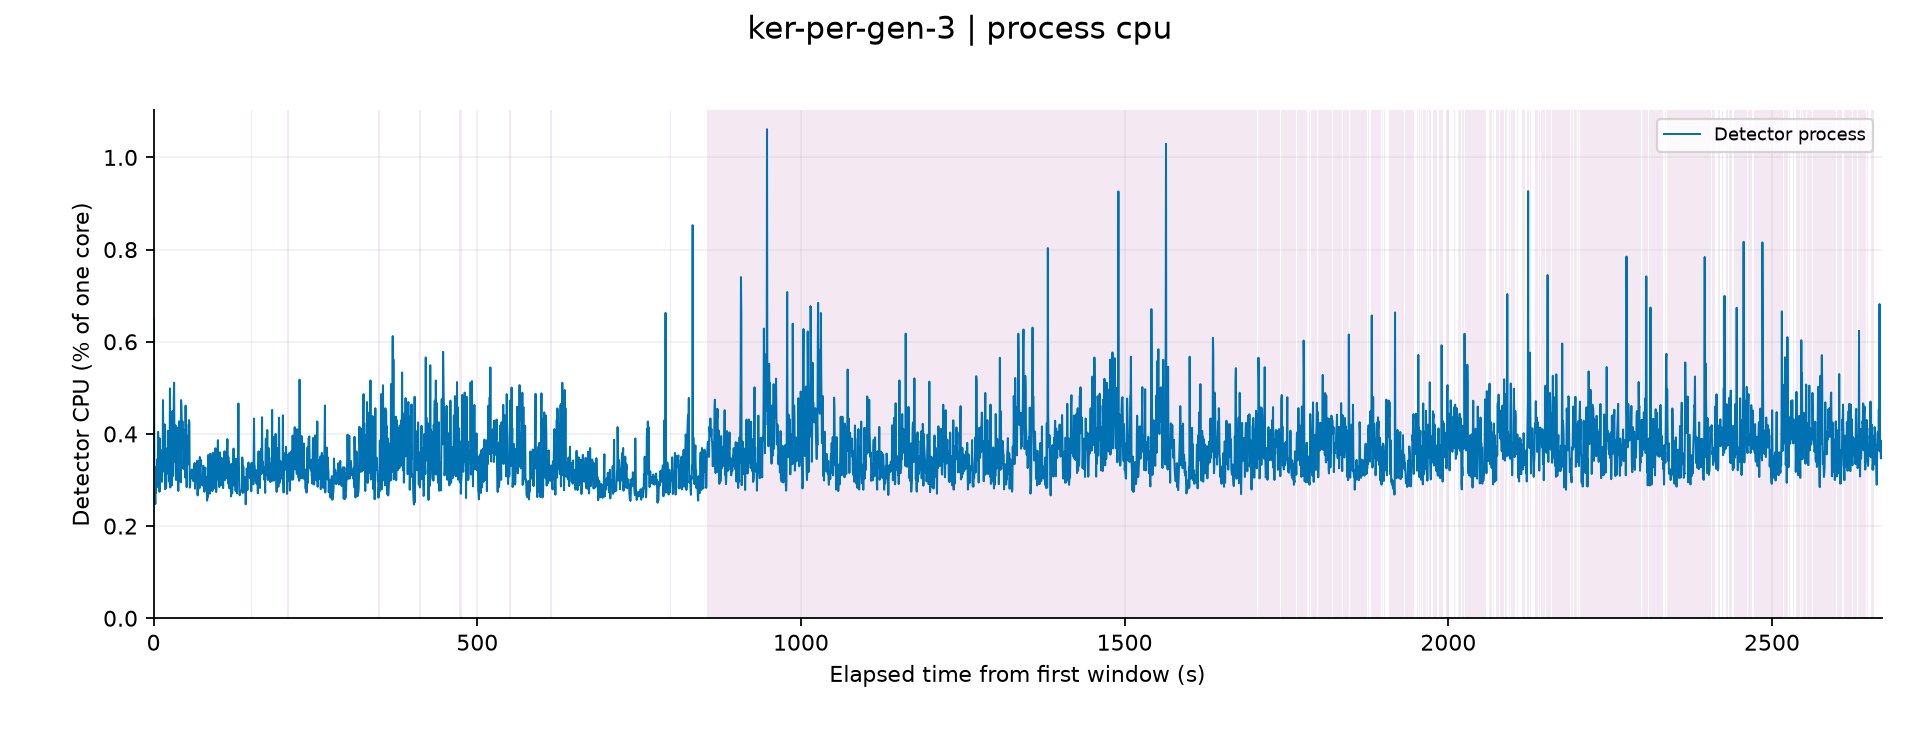
\includegraphics[width=\textwidth]{resources/testing-figures/process_cpu-ker-unblk.png}
    \caption{Detector-process CPU with blocking disabled: userspace above and kernel below. Each percentage uses one core as the denominator. XDP work is outside the kernel detector process, and the vertical scales differ substantially.}
    \label{fig:cpu-process-unblk}
\end{figure}

The userspace process closely follows the traffic load: during the flood it commonly consumes approximately 50--70\% of one core and briefly exceeds 80\%. The kernel detector process remains near 0.3--0.4\% of one core, with occasional peaks around 1\%. This demonstrates that per-packet work has moved out of the process. It does not mean that the kernel solution performs all detection work at less than 1\% CPU: the host curves include the XDP cost that the process measurement omits.

The distinction also explains why process percentages must not be directly compared with the host percentages. The two measurements have different denominators and cover different work. The offloading benefit is supported by the lower host CPU during the unblocked flood, while the much larger process-level difference primarily shows where the work executes.

\clearpage
\begin{figure}[H]
    \centering
    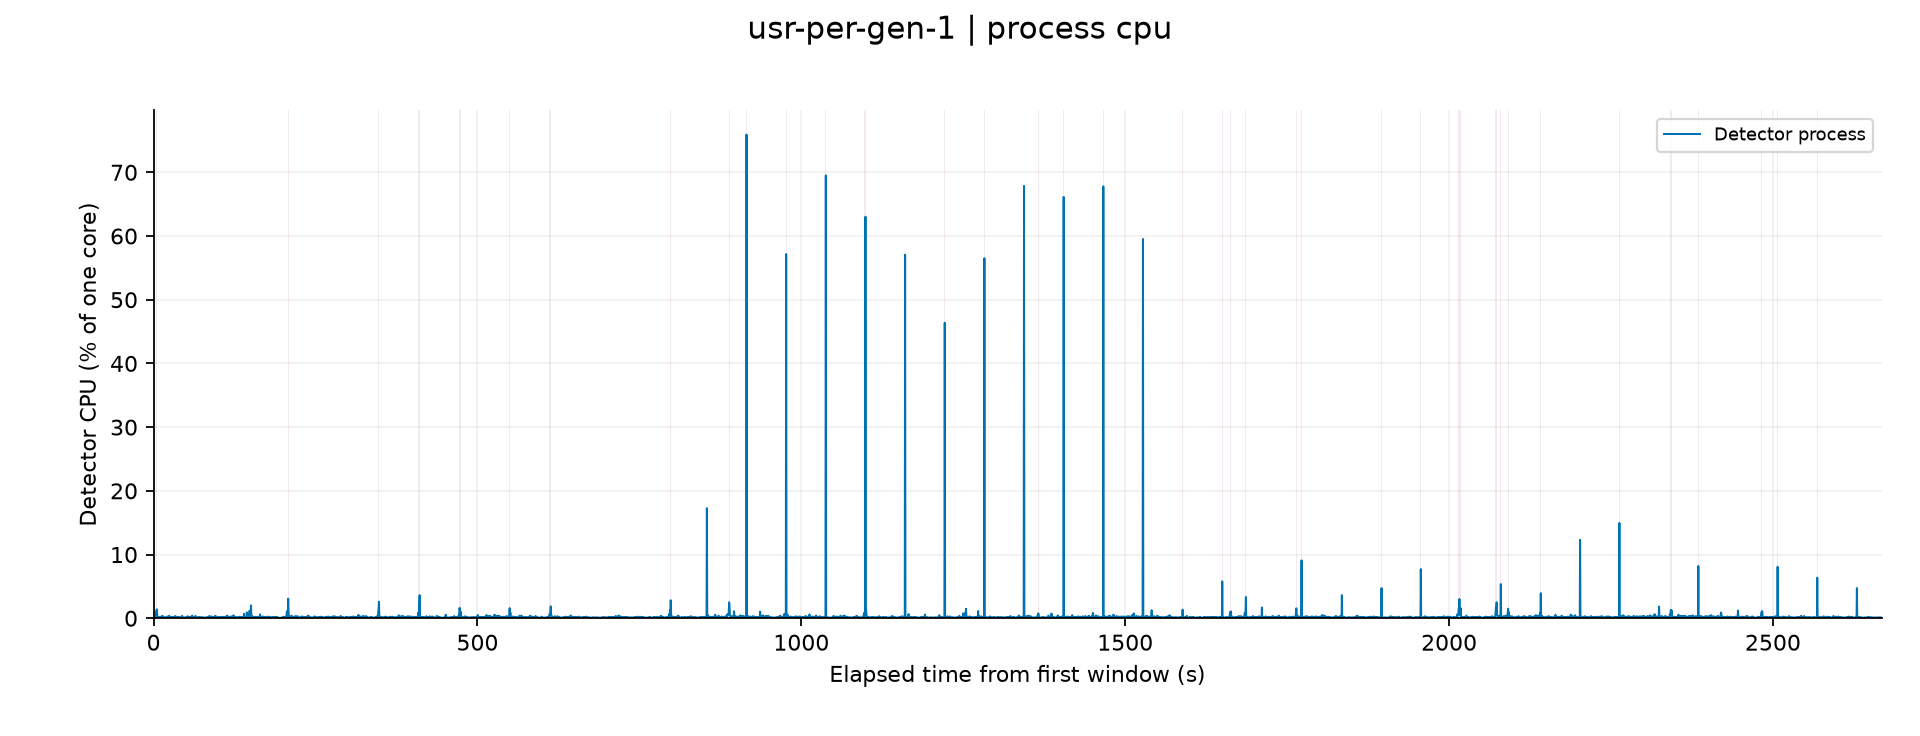
\includegraphics[width=\textwidth]{resources/testing-figures/process_cpu-usr-blk.png}
    \par\smallskip
    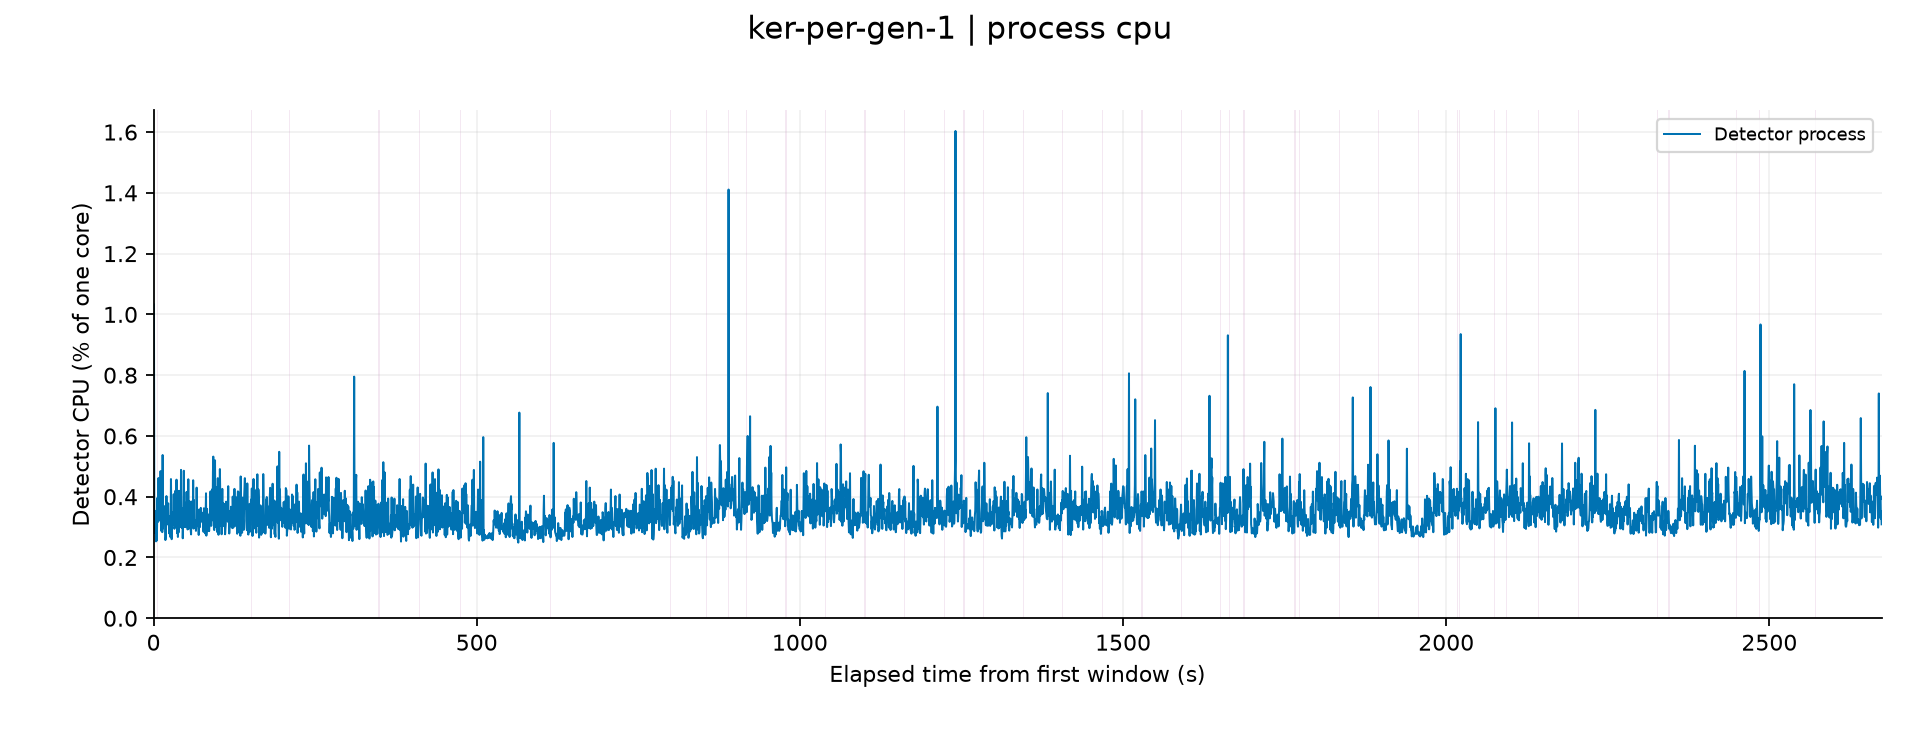
\includegraphics[width=\textwidth]{resources/testing-figures/process_cpu-ker-blk.png}
    \caption{Detector-process CPU with blocking enabled: userspace above and kernel below. Sustained utilization is low; the userspace process still experiences short bursts when traffic reaches its capture and counting path.}
    \label{fig:cpu-process-blk}
\end{figure}

With blocking enabled, the userspace process is mostly near idle but has brief peaks up to approximately 76\% of one core. The kernel process is much steadier, generally around 0.3--0.4\%, with a maximum near 1.6\%. Over the complete recordings, counter-weighted process utilization is nevertheless similar: 0.34\% for userspace and 0.35\% for the kernel detector. The main process-level difference in this scenario is the size of transient bursts, rather than a lower average for kernel detection.

\clearpage
\subsection{Throughput and packet accounting}

The throughput measurements describe observed local traffic rates at the supplied workload. They are not measurements of maximum sustainable capacity or application goodput. Table~\ref{tab:throughput} compares the two unblocked resource recordings. The complete-recording means include quiet traffic and startup. The sustained rates use each recording's highest packet-rate interval of 112 complete windows, corresponding to 60.13~s; the byte rate is calculated over that same selected interval.

\begin{table}[H]
    \centering
    \small
    \begin{tabular}{lrrr}
        \toprule
        Implementation & Mean (Mbps) & Best 60.13~s (Mbps) & Best 60.13~s (kpps) \\
        \midrule
        Userspace & 112.687 & 494.096 & 128.642 \\
        Kernel & 112.825 & 497.905 & 129.633 \\
        \bottomrule
    \end{tabular}
    \caption{Observed counted traffic with blocking disabled. Mbps uses decimal frame-byte rates. Sustained intervals are selected independently, rather than aligned between recordings.}
    \label{tab:throughput}
\end{table}

The mean byte rates differ by approximately 0.12\%, and the selected sustained rates differ by approximately 0.77\%. Both implementations therefore observed a similar workload, with no demonstrated throughput-capacity improvement. The lower kernel CPU at comparable observed rates indicates lower resource use in these runs; establishing additional capacity would require a load sweep and an explicit loss or service-quality criterion.

When blocking is enabled, low counted throughput is expected because policy drops occur before the counting stage. In the displayed blocking recordings, userspace and kernel detection intentionally block 99.09\% of counted-plus-blocked packets. Their whole-recording counted means are only approximately 0.99 and 0.98~Mbps, respectively. This is evidence of filtering activity, rather than evidence that either detector can process only that byte rate. Figure~\ref{fig:traffic} shows the much larger blocked rate alongside the residual counted traffic.

Unintentional loss must be distinguished from intentional drops. The unblocked userspace resource run reports 147,310 capture-socket drops, or 0.1875\% of socket-offered packets. Kernel XDP counting has no equivalent AF\_PACKET capture socket; the absence of that counter does not establish zero network loss. NIC and upstream losses are not fully represented by the local counting and blocking totals, and sender logs were not available for an end-to-end balance.

Finally, the recordings contain no application traffic-success measurement. Blocking a large fraction of packets does not by itself prove that legitimate requests were served or that only attack packets were dropped. Such availability claims require a benign-traffic measurement during the flood.

\clearpage
\subsection{Detection latency and local decision timing}

The recordings support a comparison of internal decision timing without aligning live traffic to dataset labels. Verdict computation runs from evaluation start to evaluation end. Window-end-to-verdict delay runs from the observation window's end until evaluation ends, including window closing, scheduling and computation. Neither measures attack-onset-to-detection latency or per-packet forwarding delay.

\begin{figure}[H]
    \centering
    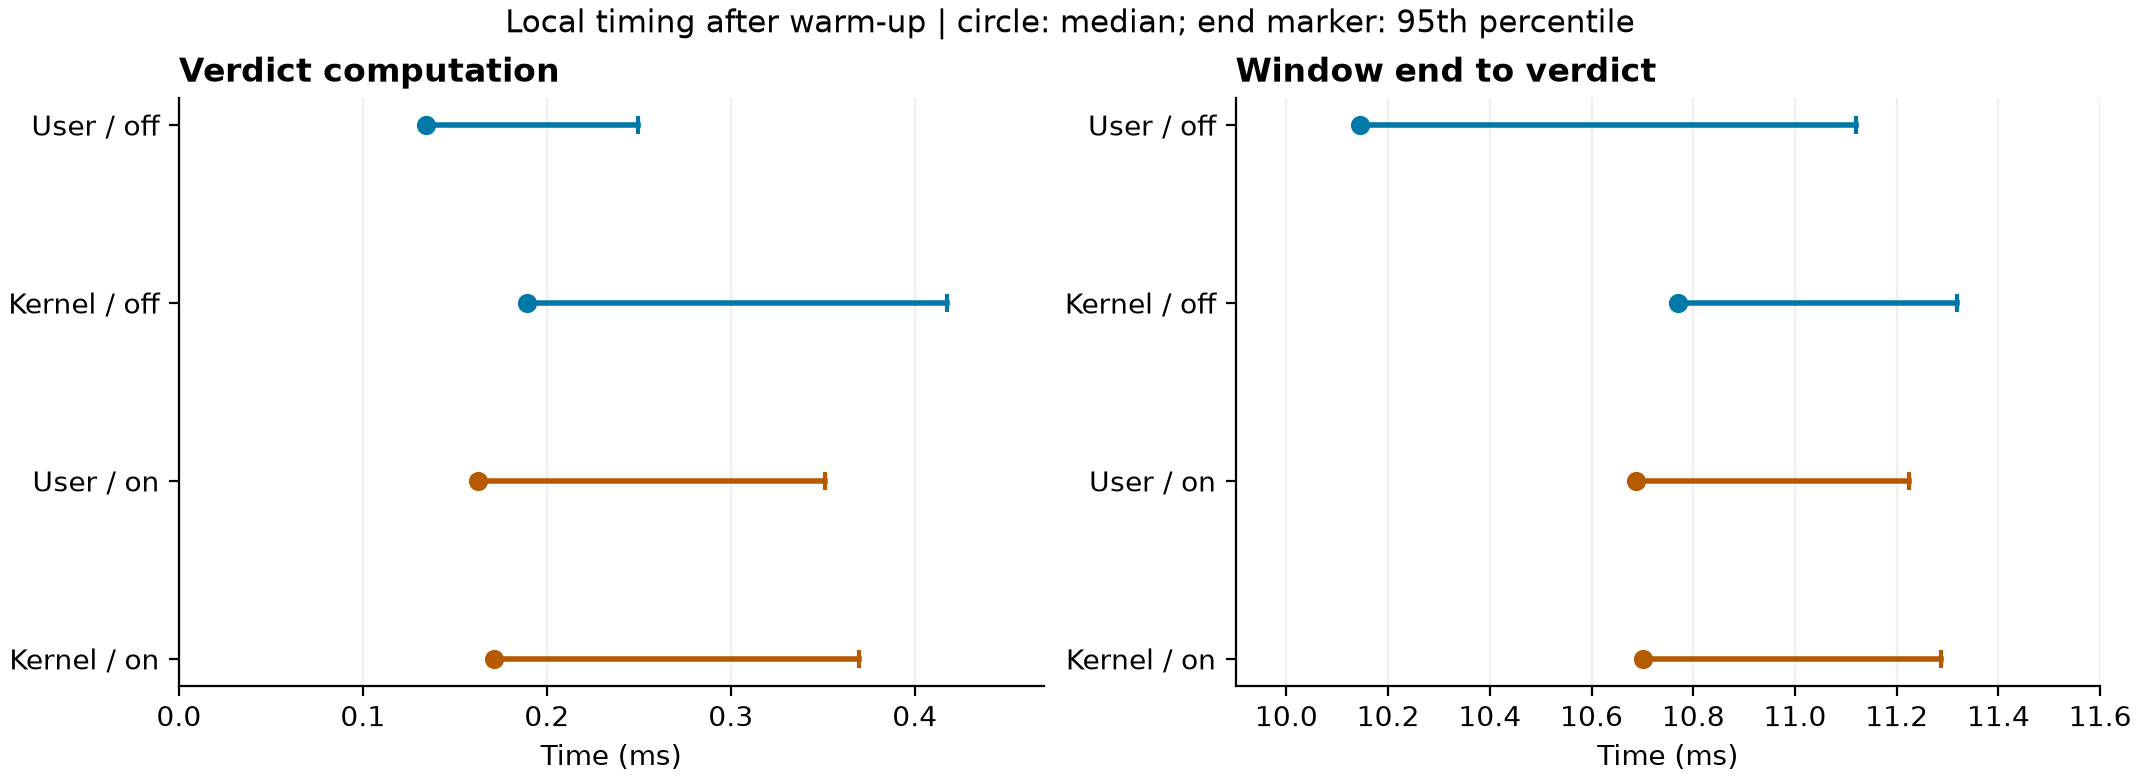
\includegraphics[width=\textwidth]{resources/testing-figures/local-latency.png}
    \caption{Local timing in the four resource recordings, using evaluated windows with \texttt{warm\_up=false}. Circles show medians and end markers show the 95th percentiles. The two panels use different horizontal scales.}
    \label{fig:local-latency}
\end{figure}

\begin{table}[H]
    \centering
    \small
    \setlength{\tabcolsep}{4pt}
    \begin{tabular}{llrrrrr}
        \toprule
        & & & \multicolumn{2}{c}{Computation (ms)} & \multicolumn{2}{c}{End to verdict (ms)} \\
        Blocking & Implementation & Windows & Median & p95 & Median & p95 \\
        \midrule
        Disabled & Userspace & 4,964 & 0.135 & 0.249 & 10.144 & 11.120 \\
        Disabled & Kernel & 4,967 & 0.189 & 0.417 & 10.770 & 11.318 \\
        Enabled & Userspace & 4,964 & 0.163 & 0.351 & 10.688 & 11.224 \\
        Enabled & Kernel & 4,975 & 0.171 & 0.370 & 10.701 & 11.287 \\
        \bottomrule
    \end{tabular}
    \caption{Local timing over each individual recording after the recorded detector warm-up. Nanosecond timestamps are subtracted as integers before conversion to milliseconds.}
    \label{tab:latency}
\end{table}

Verdict computation is sub-millisecond at the median and 95th percentile in all four recordings. Kernel computation is slightly slower in these comparisons, which is compatible with additional map-reading work after packet counting has moved to XDP. Window-end-to-verdict medians remain approximately 10--11~ms, dominated by closing and scheduling rather than the small computation interval. There is no observed improvement in that delay for the kernel implementation. The 536.87~ms observation-window duration is separate from these post-window delays.

Attack-onset latency cannot be reliably compared using the saved evaluation. The reference/live alignment fails its quality checks, so label onsets cannot be confidently placed on the live timeline. In addition, the NTP label begins approximately 3,879~s before the excerpt starts. Its saved onset-to-first-flag values of roughly 4,023--4,087~s include unobserved time before capture and do not measure a response to a newly starting attack. This onset is left-censored. DNS onset is covered, but its latency remains provisional because alignment is uncertain. These recordings therefore do not support a validated claim of improved attack-onset latency.

\clearpage
\subsection{Accuracy, precision, recall and F1 score}

Figures~\ref{fig:accuracy-user} and~\ref{fig:accuracy-kernel} compare the dataset-derived window labels with each implementation's verdicts. Grey regions are excluded or unavailable, rather than correctly classified benign windows. Table~\ref{tab:accuracy} retains the saved evaluation outputs so that their behavior can be inspected, but these figures and scores are provisional and do not provide a validated estimate of detection quality.

\begin{figure}[H]
    \centering
    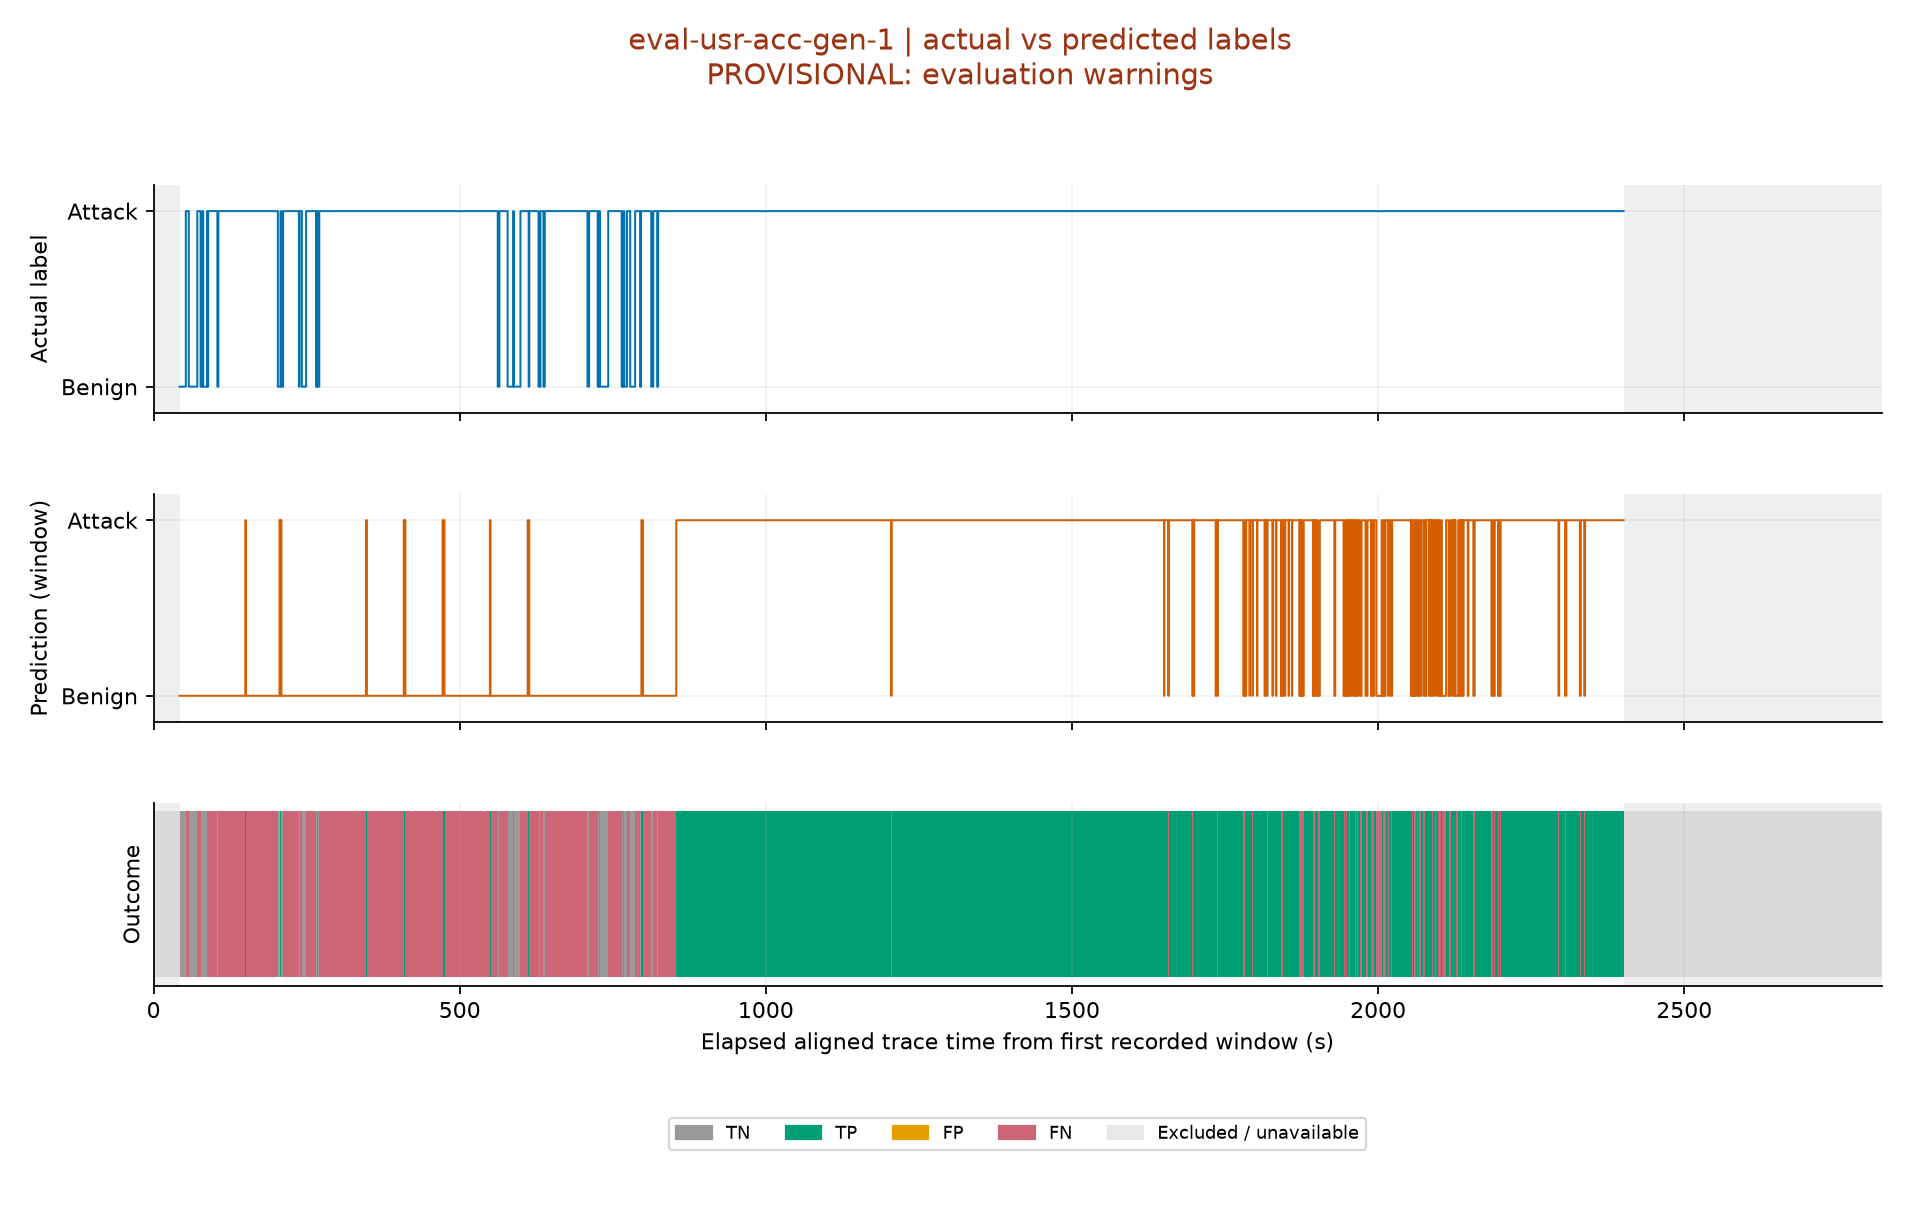
\includegraphics[width=\textwidth]{resources/testing-figures/accuracy_window-usr.png}
    \caption{Provisional userspace window-label evaluation. The top panel shows dataset-derived truth, the middle panel shows detector verdicts, and the lower strip distinguishes TP, TN, FP and FN outcomes.}
    \label{fig:accuracy-user}
\end{figure}

\begin{table}[H]
    \centering
    \small
    \begin{tabular}{lrr}
        \toprule
        Quantity & Userspace & Kernel \\
        \midrule
        True positives (TP) & 2,685 & 2,677 \\
        False positives (FP) & 5 & 7 \\
        True negatives (TN) & 228 & 226 \\
        False negatives (FN) & 1,475 & 1,483 \\
        \midrule
        Accuracy (\%) & 66.31 & 66.08 \\
        Precision (\%) & 99.81 & 99.74 \\
        Recall (\%) & 64.54 & 64.35 \\
        F1 score (\%) & 78.39 & 78.23 \\
        False-positive rate (\%) & 2.15 & 3.00 \\
        \bottomrule
    \end{tabular}
    \caption{Saved provisional scores for \texttt{eval-usr-acc-gen-1} and \texttt{eval-ker-acc-gen-1}. Each scores 4,393 windows, including 4,160 attack-labelled and 233 benign-labelled windows.}
    \label{tab:accuracy}
\end{table}

\clearpage
\begin{figure}[H]
    \centering
    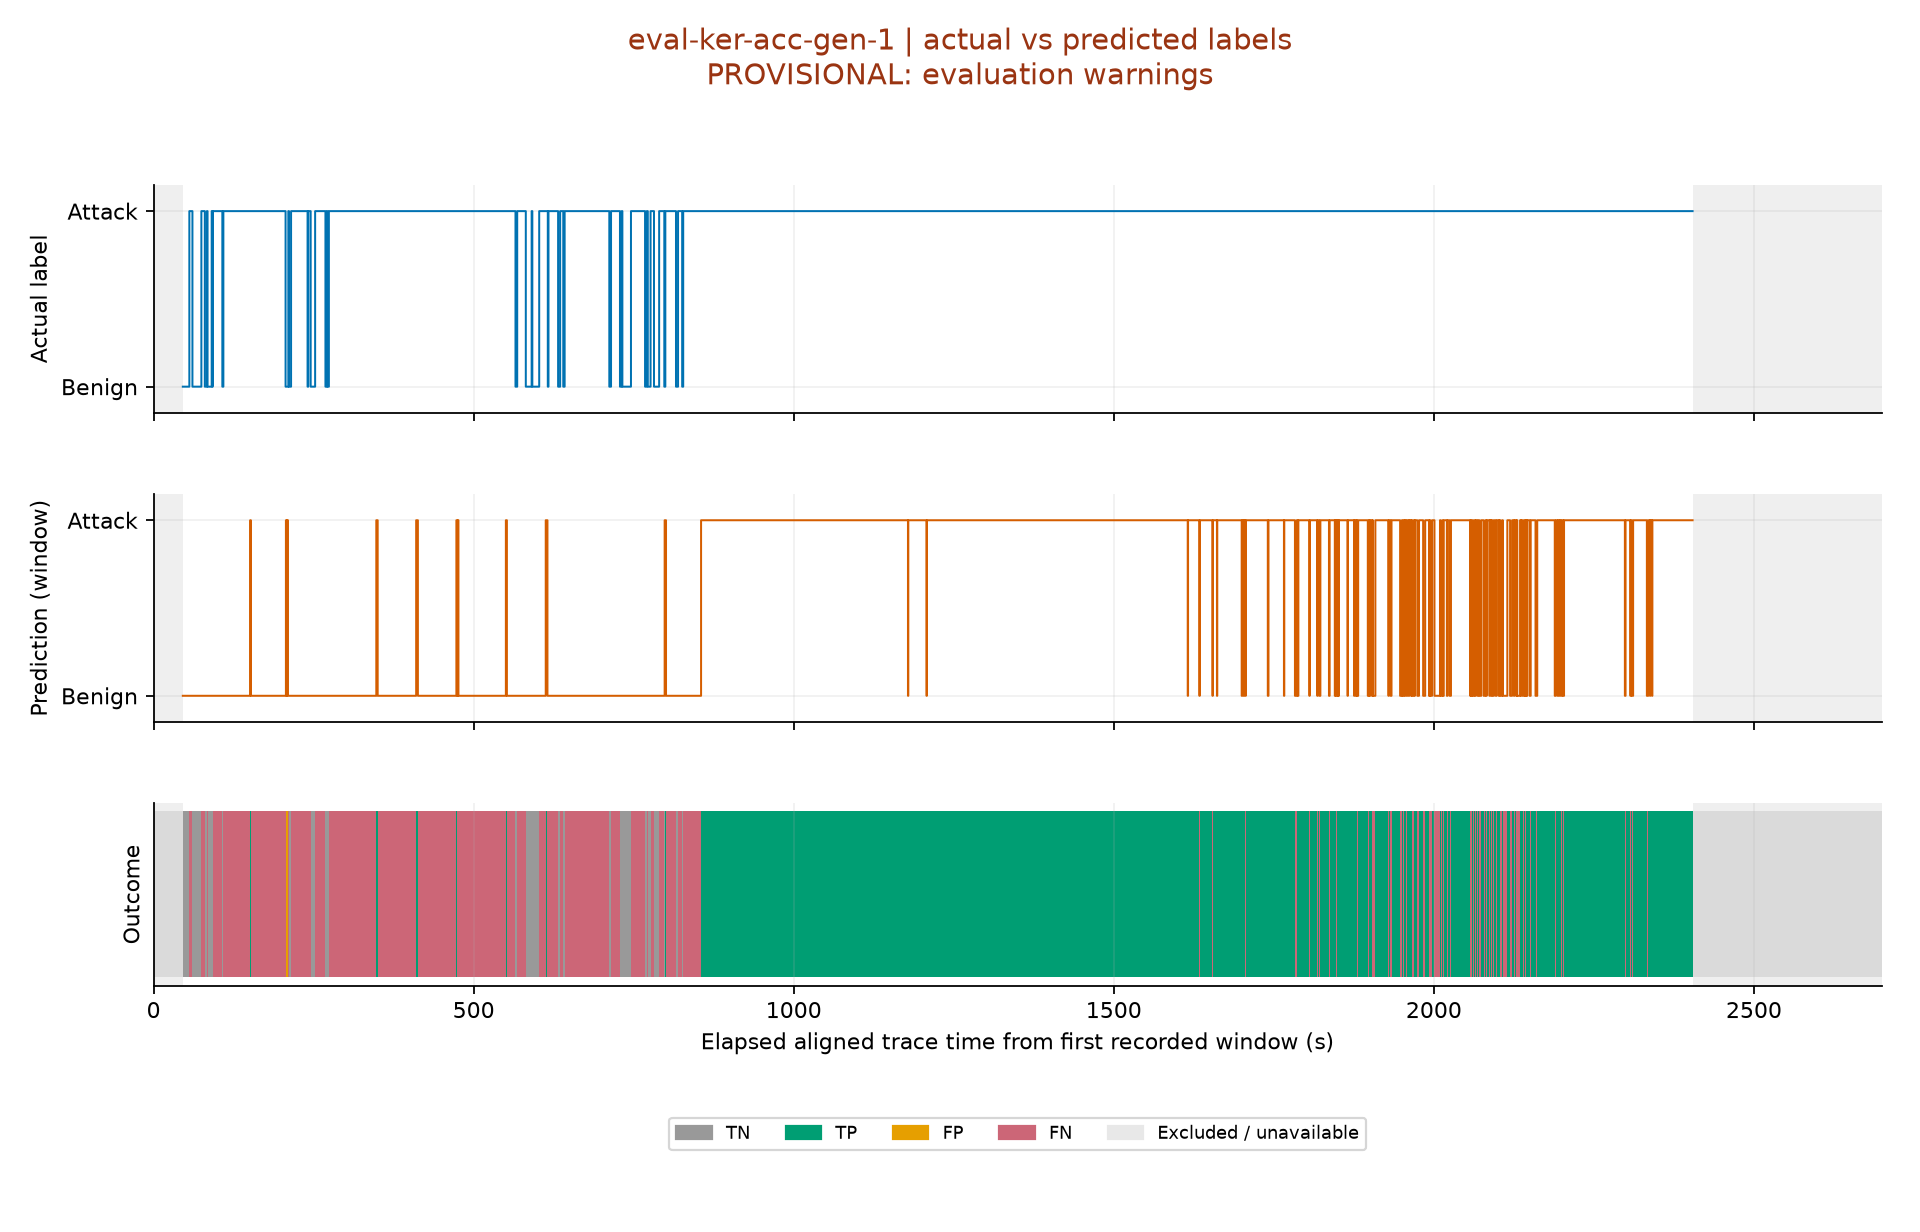
\includegraphics[width=\textwidth]{resources/testing-figures/accuracy_window-ker.png}
    \caption{Provisional kernel window-label evaluation, with the same panel definitions as Figure~\ref{fig:accuracy-user}. Similar patterns are descriptive and do not establish equivalent detection performance.}
    \label{fig:accuracy-kernel}
\end{figure}

The dominant mismatch appears before the sustained high-rate flood: many windows already carry an attack label while the detector mostly produces benign verdicts. This contributes numerous false negatives. During the large flood, both detectors produce sustained attack verdicts; verdicts become intermittent during the lower-rate tail. That response is consistent with the traffic-rate changes, but it does not establish that all missed or detected windows were correctly judged.

Two problems prevent a confident interpretation. First, the ground truth is derived from labelled flow intervals rather than packet-level onset annotations. A long attack-labelled interval can overlap a short evaluation span even when its observed rate is low. Here, 536.87~ms windows are evaluated in combined mode over approximately 1.074~s. Broad interval labels and a short-window volume detector therefore need not describe the same event. This is a limitation of this evaluation setup; it does not imply that the dataset is generally unsuitable for short-window evaluation.

Second, replay/reference timing is unvalidated. Alignment correlations of approximately 0.736--0.744 fail the evaluator's 0.9 criterion, with barely any separation between candidate offsets. The central 1--99\% packet span is approximately 1,246~s in the reference and 1,491--1,496~s live. A start-time offset cannot explain this duration difference. Replay distortion or another traffic mismatch is plausible; missing sender timing logs prevent identifying the cause. False negatives therefore cannot be attributed to the detector alone.

Class imbalance further limits the apparent high precision: approximately 94.7\% of scored windows are attack-labelled, so an always-attack prediction would already obtain 94.7\% accuracy. The 99.7--99.8\% precision must therefore be read alongside the roughly 64\% recall, confusion counts and timing problems. Similar saved scores do not establish statistical equivalence.

Only NTP and DNS have scored label coverage in this excerpt. The other ten label types are outside scored coverage and must not be reported as ten missed attacks or as a detection success rate of 2/12. A reliable detection-quality comparison requires validated replay timing and ground truth at the intended evaluation scale, followed by reevaluation of both implementations.
